\chapter{容器和字符串扩展}\label{ch26}
C++标准库的容器也有很多微小的改进,将在这一章进行讨论。


\section{节点句柄}
C++17引入了把某个节点从关联或无序容器中移入或移出的功能,使用这个功能你可以轻易地:
\begin{itemize}
    \item 修改(unordered) map的key或者(unordered) set的value
    \item 在(unordered) set和map中使用move语义
    \item 在(unordered) set和map中移动元素
    \item 把一个(unordered) set或map合并到另一个中
\end{itemize}

\subsection{修改key}
例如,考虑下面的程序:
\inputcodefile{lib/nodehandle.cpp}
在如下定义和初始化一个map之后:
\begin{lstlisting}
    std::map<int, std::string> m{{1, "mango"},
                                 {2, "papaya"},
                                 {3, "guava"}};
\end{lstlisting}
你可以像下面这样修改key \texttt{2}:
\begin{lstlisting}
    auto nh = m.extract(2); // nh的类型为decltype(m)::node_type
    nh.key() = 4;
    m.insert(std::move(nh));
\end{lstlisting}
这段代码先是把key为\texttt{2}的元素节点移出容器,然后修改了key,最后又移进了容器,
这个过程如\hyperref[f26.1]{图26.1}所示。
\begin{figure}[htb]
    \centering
    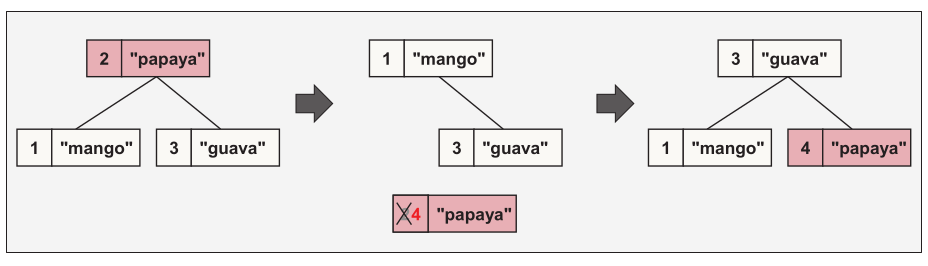
\includegraphics[scale=0.67]{../imgs/26.1.png}
    \caption{使用节点句柄修改key}
    \label{f26.1}
\end{figure}

注意在C++17之前如果想修改一个key,必须先删除旧节点然后再插入一个value相同的新节点(key是\\
\texttt{const}的,因为key的值决定了它们在容器中的位置,所以必须保持稳定)。
如果我们使用节点句柄,将不会发生内存分配,并且所有指向元素的指针和引用都保持有效,
然而,当元素还在节点句柄里而不在容器里的时候使用这些指针或者引用会导致未定义的行为。

节点句柄的类型是\emph{container}\texttt{::node\_type}。它提供了下列成员:
\begin{itemize}
    \item 所有(unordered) set类型都有\texttt{value()}成员
    \item 所有(unordered) map类型都有\texttt{key()}和\texttt{mapped()}成员
\end{itemize}

\subsection{在容器之间移动节点句柄}
你也可以使用节点句柄把一个元素从一个容器move(\emph{splice})到另一个容器。
即使容器的类型有如下不同也没有问题:
\begin{itemize}
    \item 一个支持重复而另一个不支持(例如,你可以把一个元素从multimap移动到map)
    \item 比较函数和哈希函数都不同
\end{itemize}
例如,考虑下面的程序:
\inputcodefile{lib/nodemove.cpp}
我们两次从\texttt{src}中提取元素(一次传递迭代器一次传递key)并把它们插入\texttt{dst}。
因此,程序会有如下输出:
\begin{blacklisting}
    values:
      [1.1:one]  [2.2:two]  [3.3:three]
      [3.3:old data]
    values:
      [3.3:three]
      [1.1:one]  [2.2:two]  [3.3:old data]
\end{blacklisting}
注意当不允许重复时(set、map、unordered set、unordered map),以节点句柄为参数
的\texttt{insert()}成员函数会返回一个有三个成员的结构体类型\emph{container}\texttt{::insert\_return\_type},
三个成员分别是(按照如下顺序):\label{insert节点句柄}
\begin{itemize}
    \item 一个迭代器\textbf{\texttt{position}},当插入成功时(不存在相同key的元素时)指向插入的新元素,
    当插入失败时指向已经存在的元素。
    \item 一个bool值\textbf{\texttt{inserted}}来表示插入是否成功。
    \item 一个\emph{container}\texttt{::node\_type}类型的\textbf{\texttt{node}},当插入失败时作为节点句柄。
\end{itemize}
也就是说,关键信息是第二个成员\texttt{inserted}。通过使用\nameref{ch1},你可以像下面这样使用返回值:
\begin{lstlisting}
    auto [pos, done, node] = dst.insert(src.extract(3.3));
    if (!done) {
        std::cout << "insert() of node handle failed:"
                  << " tried to insert key '" << node.key()
                  << "' with value '" << node.mapped()
                  << "' but key exists with value '" << pos->second << "'\n";
    }
\end{lstlisting}
如果一个元素被提取之后再也没有被重新插入,那么节点句柄的析构函数会释放该元素的内存。
因此,在这段代码中,即使插入失败也不会有内存泄露。

\subsection{合并容器}
以节点句柄API为基础,现在所有的关联和无序容器都提供了成员函数\texttt{merge()},
它可以把一个容器中的所有元素合并到另一个容器中。

再强调一次,即使容器的类型有如下不同也没有问题:
\begin{itemize}
    \item 一个支持重复而另一个不支持(例如,你可以把一个元素从multimap移动到map)
    \item 比较函数和哈希函数都不同
\end{itemize}
如果源容器中的某个元素因为在目标容器里已经有了key相同的元素而无法移动,
那么它会仍然留在源容器中。

例如,下面的程序:
\inputcodefile{lib/nodemerge.cpp}
会有如下输出:
\begin{blacklisting}
    values:
      [1.1:one]  [2.2:two]  [3.3:three]
      [3.3:old data]
    values:
      [3.3:three]
      [1.1:one]  [2.2:two]  [3.3:old data]
\end{blacklisting}
指向被合并元素的指针和引用仍然有效,只不过指向的容器发生了变化。


\section{emplace改进}

\subsection{emplace函数的返回类型}
对于顺序容器\texttt{std::vector<>}、\texttt{std::deque<>}、\texttt{std::list<>}和\texttt{std::forward\_list<>},
还有容器适配器\texttt{std::queue<>}和\texttt{std::stack<>},它们的emplace函数现在
返回新插入的对象的引用(关联容器以前就已经是这样了)。
这允许我们实现类似于如下的代码:
\begin{lstlisting}
    foo(myVector.emplace_back(...));
\end{lstlisting}
来代替:
\begin{lstlisting}
    myVector.emplace_back(...);
    foo(myVector.back());
\end{lstlisting}

\subsection{map的\texttt{try\_emplace()}和\texttt{insert\_or\_assign()}}
这两个成员函数让我们能够稍稍更简单或者更高效的编写处理map和unordered map的代码:
\begin{itemize}
    \item \texttt{try\_emplace()}用移动语义构造一个新的值。
    \item \texttt{insert\_or\_assign()}稍微改进了插入/更新元素的方法。
\end{itemize}

\subsection{\texttt{try\_emplace()}}
考虑下列代码:
\begin{lstlisting}
    std::map<int, std::string> m;
    m[42] = "hello";
    std::string s{"world"};
    m.emplace(42, std::move(s));    // 可能移动,但如果42已经存在时可能不会移动
\end{lstlisting}
这个调用之后\texttt{s}是否仍然保持原本的值是未定义的。
同样,对\texttt{unordered\_map}使用了\texttt{insert()}之后也是这样:
\begin{lstlisting}
    m.insert({42, std::move(s)});   // 可能移动,但如果42已经存在时可能不会移动
\end{lstlisting}
注意根据移动语义的规则这个行为并不是错误。当使用\texttt{std::move(s)}时,
我们只是表明我们对\texttt{s}的值不再感兴趣,\texttt{std::move()}会把对象标记为
可移动的但不会立刻移动走它的值。因此,在这样的调用之后,\texttt{s}\textbf{可能还有也可能没有}
原本的值了。

然而,你可能会惊讶于即使没有成功插入\texttt{s}的值也可能会被移动走(这种情况的发生和实现细节有关)。
有时,程序员可能想或者必须知道对象的值到底有没有被移走,或者想在只有插入成功时才移动走对象的值。
特别的,当使用只能移动的对象例如线程或者独占指针时就是这种情况。

例如,下面的代码是无效的,因为你必须在一个\texttt{std::thread}的析构函数被调用之前
调用它的\texttt{join()}(或者\texttt{detach()})函数:
\begin{lstlisting}
    std::map<int, std::thread> m;
    std::thread t1{...};
    m.insert({42, std::move(t1)});      // 即使没能插入也可能move
\end{lstlisting}
这里,即使\texttt{t1}没有被插入也可能会被move,这会导致core dump,
因为之后\texttt{t1}会在调用内部被销毁并且没有调用\texttt{t1.join()}。
作为代替,你可能必须像下面这样写:
\begin{lstlisting}
    auto pos = m.find(42);
    if (pos == m.end()) {
        m.insert({42, std::move(t1)});  // 如果不存在则插入(并move)
    }
\end{lstlisting}
这样写不仅代码变复杂了,还需要查找新的元素两次。

新的成员函数\texttt{try\_emplace()}保证在没有已存在元素时才会move走传入的值:
\begin{lstlisting}
    m.try_emplace(42, std::move(t1));   // 如果插入失败则不会move
\end{lstlisting}
事实上,它类似于如下写法的缩写:
\begin{lstlisting}
    auto pos = m.find(42);
    if (pos == m.end()) {
        m.emplace(42, std::move(t1));   // 插入
    }
\end{lstlisting}
不过相比之下一个好处是只会查找一次要插入的位置。

就像名字暗示的一样,\texttt{try\_emplace()}允许我们传递任意数量的参数来
在元素不存在时初始化一个新的元素:
\begin{lstlisting}
    std::map<int, std::string> ms;
    ms.try_emplace(42, "hello");    // 尝试插入元素,value为"hello"
    ms.try_emplace(43, 8, 'a');     // 尝试插入元素,value为"aaaaaaaa"
\end{lstlisting}
然而,注意你不能以这种方式初始化一个容器里的元素:
\begin{lstlisting}
    std::map<int, std::vector<std::string>> vals;
    std::string h{"hello"};
    std::string w{"world"};
    vals.try_emplace(42, std::vector<std::string>{h, w});   // OK
    vals.try_emplace(42, h, w);                             // ERROR
\end{lstlisting}
可以传递一个额外的迭代器作为第一个参数,它被用作查找新元素应该放置的位置时的提示。

\subsection{\texttt{insert\_or\_assign()}}
另外,新的成员函数\texttt{insert\_or\_assign()}保证把值移动到一个新的元素或者已存在的元素中:
\begin{lstlisting}
    m.insert_or_assgin(42, std::move(t1));  // 总是会move
\end{lstlisting}
它的行为类似于如下代码的缩写:
\begin{lstlisting}
    auto pos = m.find(42);
    if (pos == m.end()) {
        m.insert({42, std::move(t1)});  // 插入
    }
    else {
        pos->second = std::move(t1);    // 更新
    }
\end{lstlisting}
类似于
\begin{lstlisting}
    m[42] = std::move(t1);              // key不存在时首先默认初始化value,再覆盖value
\end{lstlisting}
不过相比之下的好处是新元素的位置只会查找一次,并且新元素并不是首先用默认构造函数构造然后再覆写。

因此,这个成员函数可以在默认构造函数不能调用的情况下允许我们插入或者更新一个元素。

注意\texttt{insert\_or\_assign()}把key和value作为分离的参数,而\texttt{insert()}
把它们作为一个整体参数。
另外,可以传递一个额外的迭代器作为第一个参数,它被用作查找新元素应该放置的位置时的提示。


\section{对不完全类型的容器支持}
自从C++17起,\texttt{std::vector}、\texttt{std::list}、\texttt{std::forward\_list}被要求支持
不完全类型。

这个特性的主要动机在Matt Austern的一篇标题
为\emph{The Standard Librarian: Containers of Incomplete Types}
的文章中进行了解释:
\footnote{见\url{See http://web.archive.org/web/20190305220304/http://www.drdobbs.com/184403814}。}
你现在可以定义一个类型,内部递归的包含一个自身类型的容器。例如:
\begin{lstlisting}
    struct Node
    {
        std::string value;
        std::vector<Node> children; // 自从C++17起OK(这里Node是一个不完全的类型)
    };
\end{lstlisting}
这也适用于带有private成员和public API的类。
这里有一个完整的例子:
\inputcodefile{lib/incomplete.hpp}
你可以像下面这样使用这个类:
\inputcodefile{lib/incomplete.cpp}
程序会有如下输出:
\begin{blacklisting}
    top
      elem1
        elem1.1
      elem2
\end{blacklisting}


\section{string改进}
对于string(类型为\texttt{basic\_string<>)},C++17提供了以下一些改进:
\begin{itemize}
    \item 对于非常量string,你现在也可以调用\texttt{data()}把底层的字符序列当作原生C字符串来访问:
    \begin{lstlisting}
    std::string mystring{"Hello world"};
    auto cstr = mystring.data();
    cstr[6] = 'W';                      // 自从C++17起OK
    \end{lstlisting}
    注意在C++17之前,\texttt{cstr}的类型将是\texttt{const char*},而现在它的类型是\texttt{char*}。
    在C++17之前,把\texttt{data()}的返回值赋值给\texttt{char*}将不能通过编译:
    \begin{lstlisting}
    std::string mystring{"Hello world"};
    char* cstr = mystring.data();   // 自从C++17起OK
    \end{lstlisting}
    和以前一样,只要\texttt{std::string}还存在并且没有重新分配内存,
    对\texttt{data()}的返回值的访问就是有效的。修改\texttt{data()}返回值的末尾的空终止符仍然是未定义行为。
    \item 还提供了一个到\texttt{std::string\_view}的隐式转换,然而,这可能会导致一些bug或者歧义。
    见\hyperref[ch19]{关于字符串视图的章节}获取详情。
    \item 字符串现在也支持多态类型资源,这意味着你可以声明:
    \begin{lstlisting}
    std::pmr::string s1;
    std::pmr::wstring s1;
    std::pmr::u16string s1;
    std::pmr::u32string s1;
    \end{lstlisting}
    见\hyperref[ch29]{PMR章节}获取详情。
\end{itemize}


\section{后记}
Alan Talbot在\url{https://wg21.link/lwg839}中要求拼接操作、
Alisdair Meredith在\url{https://wg21.link/lwg1041}中要求节点元素要有更多操作支持,
这两个提案都是作为标准库的issue提出,间接的首次提出了节点句柄的概念。

最终被接受的是Alan Talbot、Jonathan Wakely、Howard Hinnant、James Dennett
发表于\url{https://wg21.link/p0083r3}的提案。
Howard E. Hinnant在\url{https://wg21.link/p0508r0}中稍微修改使API更加明晰,并成为了最终版本的API。

emplace成员函数的新返回值类型由Alan Talbot在\url{https://wg21.link/p0084r0}中首次提出。
最终被接受的是Alan Talbot发表于\url{https://wg21.link/p0084r2}的提案。

(unordered) map的\texttt{insert\_or\_assign()}和\texttt{try\_emplace()}操作由
Thomas Köppe在\url{https://wg21.link/n3873}中首次提出。
最终被接受的是Thomas Köppe发表于\url{https://wg21.link/n4279}的提案。

对不完全类型的容器支持由Matt Austern在\url{http://drdobbs.com/184403814}中首次讨论,
由Zhihao Yuan在\url{https://wg21.link/n3890}中首次提出。
最终被接受的是Zhihao Yuan发表于\url{https://wg21.link/n4510}的提案。

string的\texttt{data()}支持由Michael Bradshaw在\url{https://wg21.link/lwg2391}
中作为标准库的issue首次提出。最终被接受的是David Sankel发表于\url{https://wg21.link/p0272r1}的提案。
